\documentclass[xcolor=dvipsnames]{beamer} 
\usepackage{graphicx}
\usepackage{tikz}
\usetikzlibrary{matrix,arrows}
% \usepackage{pgfbaselayers}
% \pgfdeclarelayer{background}
% \pgfdeclarelayer{foreground}
% \pgfsetlayers{background,main,foreground}

%\includeonlyframes{titlepage,background,algebras,algexamples,lattices,distributivity,%
%eqlat,conglat2,congruences,conglat1,groupcong,subglat,hasseexample,info,flrp}
%\includeonlyframes{eqlatex,concrete,galois,closure}
%\includeonlyframes{info,closure,results}
%\includeonlyframes{results,results2,results3,results4,results5,summary}

%\usepackage{enumerate,amsmath,amssymb,fancyhdr,mathrsfs,amsthm}
\usepackage{mathrsfs,textcomp}
%\documentclass[draft]{beamer} 
%\documentclass{beamer} 
\setbeamertemplate{navigation symbols}{}
\usepackage{verbatim}
\usepackage[mathcal]{euscript}

\usecolortheme[named=OliveGreen]{structure} 
\setbeamertemplate{items}[ball] 
\setbeamertemplate{blocks}[rounded][shadow=true] 
% - Talk at a conference/colloquium.
% - Talk length is about 20min.
% - Style is ornate.

% This changes the color of alerted text to blue:
\definecolor{MyDarkBlue}{rgb}{0.2,0.2,0.7}
\definecolor{olivegreen}{cmyk}{0.64,0,0.95,0.40} % PANTONE 582
\setbeamercolor{alerted text}{fg=blue}
\newcommand{\emphcyan}[1]{\textcolor{MyDarkBlue}{\textbf{#1}}}
%\renewcommand{\alert}[1]{\textcolor{MyDarkBlue}{\emph{#1}}}
% (default is red, but my slides are green and I don't like red and green together)


\newcommand{\Hawaii}{Hawai\kern.05em`\kern.05em\relax i}
\newcommand{\Manoa}{M\=anoa}
\newcommand{\cd}{\ensuremath{\otimes}}
\newcommand{\con}[1]{\ensuremath{\langle #1 \rangle}}
\newcommand{\ii}[1]{{\it #1}}
\newcommand{\power}[1]{\ensuremath{\mathscr{P}(#1)}}
\newcommand{\scrA}{\ensuremath{\mathscr{A}}}
\newcommand{\bM}{\ensuremath{\mathbf{M}}}
\newcommand{\Mn}{\ensuremath{\mathbf{M}_n}}
\newcommand{\bF}{\ensuremath{\mathbf{F}}}
\newcommand{\bE}{\ensuremath{\mathbf{E}}}
\newcommand{\bR}{\ensuremath{\mathbf{R}}}
\newcommand{\bA}{\ensuremath{\mathbf{A}}}
\newcommand{\bG}{\ensuremath{\mathbf{G}}}
\newcommand{\bH}{\ensuremath{\mathbf{H}}}
\newcommand{\bK}{\ensuremath{\mathbf{K}}}
\newcommand{\bL}{\ensuremath{\mathbf{L}}}
\newcommand{\bB}{\ensuremath{\mathbf{B}}}
\newcommand{\svert}{\ensuremath{\; \vert \; }}

\newcommand{\sE}{\ensuremath{\mathcal{E}}}
\newcommand{\sH}{\ensuremath{\mathcal{H}}}
\newcommand{\sS}{\ensuremath{\mathcal{S}}}
\newcommand{\sL}{\ensuremath{\mathcal{L}}}
\newcommand{\bN}{\ensuremath{\mathbf{N}}}
\newcommand{\bX}{\ensuremath{\mathbf{X}}}


\newcommand{\sA}{\ensuremath{\mathcal{A}}}
\newcommand{\sB}{\ensuremath{\mathcal{B}}}
\newcommand{\sC}{\ensuremath{\mathcal{C}}}
\newcommand{\SSS}{\text{\emphslb{S}}}
\newcommand{\id}{\mbox{id}}
\newcommand{\Hom}{\mbox{Hom}}
\newcommand{\End}{\ensuremath{\mathrm{End}}}
\newcommand{\bEnd}{\ensuremath{\mathbf{End}}}
\newcommand{\Aut}{\ensuremath{\mathrm{Aut}}}
\newcommand{\bAut}{\ensuremath{\mathbf{Aut}}}
\newcommand{\Con}{\ensuremath{\mathrm{Con}}}
\newcommand{\bCon}{\ensuremath{\mathbf{Con}}}
\newcommand{\Sub}{\mbox{Sub}}
\newcommand{\bSub}{\ensuremath{\mathbf{Sub}}}
\newcommand{\CSub}[1]{\ensuremath{\mathbf{CSub}[#1]}}
\newcommand{\csub}{\ensuremath{\mbox{CSub}}}
\newcommand{\Stab}{\mbox{Stab}}
\newcommand{\bStab}{\ensuremath{\mathbf{Stab}}}
\newcommand{\X}{\ensuremath{\mathbf{X}}}
\newcommand{\image}{\mbox{im}}
\newcommand{\Eq}{\mbox{Eq}}
\newcommand{\bEq}{\ensuremath{\mathbf{Eq}}}
\newcommand{\bEqX}{\ensuremath{\mathbf{Eq}(X)}}
\newcommand{\idemdec}{\ensuremath{\mbox{Idemdec}(X)}}
\newcommand{\EqX}{\ensuremath{\mbox{Eq}(X)}}
\newcommand{\upalpha}{\ensuremath{\alpha^{\uparrow}}}
\newcommand{\downalpha}{\ensuremath{\alpha^{\downarrow}}}
\newcommand{\upbeta}{\ensuremath{\beta^{\uparrow}}}
\newcommand{\downbeta}{\ensuremath{\beta^{\downarrow}}}
\newcommand{\meet}{\ensuremath{\wedge}}
\newcommand{\join}{\ensuremath{\vee}}
\newcommand{\Meet}{\ensuremath{\bigwedge}}
\renewcommand{\Join}{\ensuremath{\bigvee}}

%%% Freese Macros %%%
%%%=================Emphasizing with bold=================

%\DeclareRobustCommand\emb
%        {\@nomath\emb \ifdim \fontdimen\@ne\font >\z@
%                       \upshape \else \bfseries \fi}
%
%
%\DeclareTextFontCommand{\emphb}{\emb}

%\DeclareRobustCommand\emslb
%        {\@nomath\emb \ifdim \fontdimen\@ne\font >\z@
%                       \bfseries\slshape \else \bfseries\slshape \fi}
\DeclareRobustCommand\emslb{\bfseries\slshape}
\DeclareTextFontCommand{\emphslb}{\emslb}
\newcommand{\alg}[1]{\mathbf{#1}}
\newcommand{\HH}{\text{\emphslb{H}}}
\renewcommand{\SS}{\text{\emphslb{S}}}
\newcommand{\PP}{\text{\emphslb{P}}}
\newcommand{\II}{\text{\emphslb{I}}}
\newcommand{\VV}{\text{\emphslb{V}}}
\newcommand{\vr}{\VV}
\newcommand{\Ps}{\PP_{\text{\emphslb{s}}}}
\newcommand{\Si}{\SS_{\text{\emphslb{i}}}}
\renewcommand{\Pr}{\PP_{\text{\emphslb{r}}}}
\newcommand{\Pu}{\PP_{\text{\emphslb{u}}}}
\newcommand{\Se}{\SS^{\prec}}
\newcommand{\urt}{\sqrt[\text{\emphslb{u}}]}
\newcommand{\la}{\langle}	     %% left angle for order sequences <a,b>
\newcommand{\ra}{\rangle}	     %% right angle

\newcommand{\<}{\langle}	     %% left angle for order sequences <a,b>
\renewcommand{\>}{\rangle}	     %% right angle
\newcommand{\algA}{\ensuremath{\<A, F\>}}

 \mode<presentation>
 {
%   \setbeamertemplate{background canvas}[vertical shading][bottom=green!10,top=gray!10]
%   \usetheme{Warsaw}
   \usetheme{Madrid}
   % or ...
   %\setbeamercovered{transparent}
   % or whatever (possibly just delete it)
 }

\usepackage[english]{babel}
\usepackage[latin1]{inputenc}
\usepackage{times}
\usepackage[T1]{fontenc}
% Or whatever. Note that the encoding and the font should match. If T1
% does not look nice, try deleting the line with the fontenc.

\title[Finite Lattice Representation Problem] % (optional, will appear at bottom of each slide)
{The Finite Lattice Representation Problem}
%\subtitle{intervals in subgroup lattices and \\ the dawn of tame congruence theory}


\author[William DeMeo]{William DeMeo\\
{\tiny joint work with}\\ 
{\small Ralph Freese, Peter Jipsen, Bill Lampe, J.B. Nation}}
%\institute[University of \Hawaii]%
%{University of \Hawaii\ at \Manoa}
\institute[UH Math]{University of \Hawaii\ at \Manoa}

\date[ARCS 2011]% (optional, should be abbreviation of conference name)
{ARCS Presentation\\
April 23, 2011}
%\date[Honolulu 2009]{Math 613: Group Theory\\ November 2009}

\subject{Universal Algebra; Lattice Theory.}% (optional) inserted into PDF info catalog.

% TOC pops up at the beginning of each subsection:
\AtBeginSubsection[]
{
  \begin{frame}<beamer>
    \frametitle{Outline}
    \tableofcontents[currentsection,currentsubsection]
  \end{frame}
}

% If you wish to uncover everything in a step-wise fashion, uncomment the following command: 
% \beamerdefaultoverlayspecification{<+->}

\begin{document}
\thicklines

\frame[label=titlepage]{
  \titlepage
}


%% 2.  %%%%%%%%%%%%%%%%%%%%%%%%%%%%%%%%%%%%%%%%%%%%%%%%%%%%%%%%%%%%%%%%%%%%%%%%%%%%%
\frame[label=apology]{
  \frametitle{Apology}
  \begin{center}
  \uncover<1->{I am sorry...\\[8pt]}
  \uncover<2->{...this talk is about math.}
  \end{center}
}

%% 3.  %%%%%%%%%%%%%%%%%%%%%%%%%%%%%%%%%%%%%%%%%%%%%%%%%%%%%%%%%%%%%%%%%%%%%%%%%%%%%
\frame[label=algebras]{
  \frametitle{What is an algebra?}
  \framesubtitle{...an utterly fundamental object in mathematics.}
  \uncover<1->{  
  \begin{definition}
    An \alert{algebra} $\bA$ is an ordered pair $\bA = \langle A, F\rangle$ where}
    \begin{itemize}
    \item<2->[] $A$ is a nonempty set, called the \emph{universe} of \bA
    \item<2->[] $F$ is a family of operations acting on $\bA$
    \end{itemize}
    \uncover<3->{An algebra $\langle A, F \rangle$ is called \alert{finite} if $|A|$ is finite.}
  \end{definition}

  \begin{itemize}
  \item<4->
    {\bf Example:} The set of integers 
    \[A = \{\dots, -2, -1, 0, 1, 2, \dots\}\]
    \uncover<5->
    {along with the operations $F = \{+, -, \times\}$.}
    \uncover<6>
    {~\\[8pt]{\it Question:} Is $\div$ an operation on this set, $A$?}
  \item<7->\vspace{-1em}
    {\bf Other Examples:} semigroups, groups, quasigroups, rings, modules,
    lattices, Boolean algebras, $*$-algebras, etc.
  \end{itemize}
}

%% 4.  %%%%%%%%%%%%%%%%%%%%%%%%%%%%%%%%%%%%%%%%%%%%%%%%%%%%%%%%%%%%%%%%%%%%%%%%%%%%%
\frame[label=algexamples]{
  \frametitle{Examples}
  \begin{itemize}
  \item<1->
    A \alert{lattice} is an algebra $\bL = \langle L, \meet, \join\rangle$ with
    universe $L$ %, a partially ordered set, 
    and binary operations:
    \begin{itemize}
    \item<2->[] $x\meet y = \text{g.l.b.}(x,y)$ \phantom{x} the ``meet'' of $x$ and $y$
    \item<2->[] $x\join y = \text{l.u.b.}(x,y)$ \phantom{x} the ``join'' of $x$ and $y$
    \end{itemize}

    \vspace{.5em}

  \item<3->{\it Examples of lattices:}
    \uncover<3>{
      \begin{itemize}
      \item subsets of a set    
      \item closed subsets of a topology
      \item  subgroups of a group, normal subgroups of a group
      \item ideals of a ring 
      \item submodules of a module 
      \item invariant subspaces of an operator or operator algebra
      \end{itemize}
    }
    \uncover<4>{
      
      \vspace{-7em}
      \begin{center}
        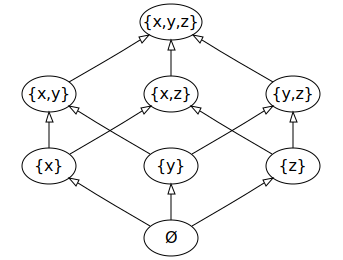
\includegraphics[height=1.9in]{PowerSet3}
      \end{center}
    }
    \uncover<5>{
      
      \vspace{-14em}
      \begin{center}
        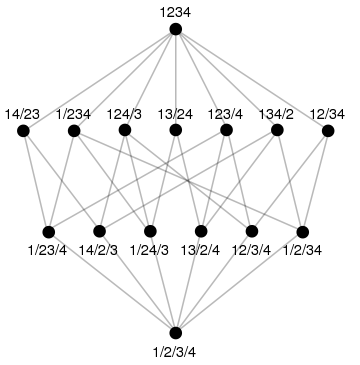
\includegraphics[height=1.9in]{360px-Lattice_of_partitions_of_an_order_4_set}
      \end{center}
}
  \end{itemize}
}

%% 5.  %%%%%%%%%%%%%%%%%%%%%%%%%%%%%%%%%%%%%%%%%%%%%%%%%%%%%%%%%%%%%%%%%%%%%%%%%%%%%
%%%% Freese Frame -- Lattices explained by Hasse diagram %%
\frame[label=lattices]{
  \frametitle{Lattices}
\begin{center}
\hspace{3cm}
\setlength{\unitlength}{0.9cm}
\begin{picture}(6,8)

\put(0,0){\circle*{0.15}}
\put(-1,1){\circle*{0.15}}
\put(1,1){\circle*{0.15}}
\put(0,1){\circle*{0.15}}
\put(-1,2){\circle*{0.15}}
\put(1,2){\circle*{0.15}}
\put(0,2){\circle*{0.15}}
\put(0,3){\circle*{0.15}}
%%%%%
\put(0,0){\line(1,1){1}}
\put(0,0){\line(-1,1){1}}
\put(0,0){\line(0,1){1}}
\put(-1,1){\line(0,1){1}}
\put(-1,1){\line(1,1){1}}
\put(1,1){\line(0,1){1}}
\put(1,1){\line(-1,1){1}}
\put(0,1){\line(1,1){1}}
\put(0,1){\line(-1,1){1}}
\put(-1,2){\line(1,1){1}}
\put(1,2){\line(-1,1){1}}
\put(0,2){\line(0,1){1}}
%%%%%
%\put(0,4){\circle*{0.15}}
\put(1,4){\circle*{0.15}}
\put(-1,4){\circle*{0.15}}
%%%%%
\put(0,3){\line(1,1){1}}
\put(0,3){\line(0,1){1}}
\put(0,3){\line(-1,1){1}}
\put(0,4){\line(0,1){1}}
\put(1,4){\line(-1,1){1}}
\put(-1,4){\line(1,1){1}}
%%%%%
\put(0,5){\circle*{0.15}}
\put(-1,6){\circle*{0.15}}
\put(1,6){\circle*{0.15}}
\put(0,6){\circle*{0.15}}
\put(-1,7){\circle*{0.15}}
\put(1,7){\circle*{0.15}}
\put(0,7){\circle*{0.15}}
\put(0,8){\circle*{0.15}}
%%%%%
\put(0,5){\line(1,1){1}}
\put(0,5){\line(-1,1){1}}
\put(0,5){\line(0,1){1}}
\put(-1,6){\line(0,1){1}}
\put(-1,6){\line(1,1){1}}
\put(1,6){\line(0,1){1}}
\put(1,6){\line(-1,1){1}}
\put(0,6){\line(1,1){1}}
\put(0,6){\line(-1,1){1}}
\put(-1,7){\line(1,1){1}}
\put(1,7){\line(-1,1){1}}
\put(0,7){\line(0,1){1}}
%%%%%
\put(3,4){\circle*{0.15}}
\put(2,5){\circle*{0.15}}
\put(2,3){\circle*{0.15}}
\put(-3,4){\circle*{0.15}}
\put(-2,5){\circle*{0.15}}
\put(-2,3){\circle*{0.15}}
%%%%%
\put(3,4){\line(-1,1){1}}
\put(2,5){\line(-1,1){1}}
\put(2,3){\line(-1,1){1}}
\put(2,3){\line(1,1){1}}
\put(1,4){\line(1,1){1}}
\put(1,2){\line(1,1){1}}

\put(-3,4){\line(1,1){1}}
\put(-2,5){\line(1,1){1}}
\put(-2,3){\line(1,1){1}}
\put(-2,3){\line(-1,1){1}}
\put(-1,4){\line(-1,1){1}}
\put(-1,2){\line(-1,1){1}}

\textcolor{red}{
\put(0,4){\circle*{0.15}}
\put(-2,4){\circle*{0.15}}
\put(-1,5){\circle*{0.15}}
\put(-1,3){\circle*{0.15}}
\put(-2,4){\line(1,1){1}}
\put(-1,5){\line(1,1){1}}
\put(-1,3){\line(1,1){1}}
\put(-1,3){\line(-1,1){1}}
\put(0,4){\line(-1,1){1}}
\put(0,2){\line(-1,1){1}}
}
\uncover<3>{
\put(-1,3){\textcolor{yellow}{\line(1,1){1}}}
\put(0,4){\textcolor{yellow}{\line(0,1){1}}}
\put(0,5){\textcolor{yellow}{\line(1,1){1}}}
\put(1,6){\textcolor{yellow}{\line(0,1){1}}}
}
\uncover<3>{
\put(3.5,5.5){\Large\textbf{$v \leq w$}}
}
\uncover<2->{
\put(-1,3){\textcolor{blue}{\circle*{0.2}}}
\put(-1.2,2.9){\textbf{\llap{$v$}}}
\put(1,7){\textcolor{green}{\circle*{0.2}}}
\put(1.2,6.9){\textbf{$w$}}
}
\uncover<4->{
\put(3,4){\textcolor{blue}{\circle*{0.2}}}
\put(3.2,3.9){\textbf{$z$}}
}
\uncover<4>{
\put(3.5,5.5){\textbf{\Large$v \nleq z$}}
}
\uncover<5->{
\put(1.2,5.9){\textbf{$v \join z$}}
}
\uncover<6->{
\put(-3,4){\textcolor{blue}{\circle*{0.2}}}
\put(-3.2,3.9){\textbf{\llap{$x$}}}
\put(-2,4){\textcolor{blue}{\circle*{0.2}}}
\put(-2.2,3.9){\textbf{\llap{$y$}}}
}
\uncover<6>{
\put(3.5,5.5){\textbf{\Large$x$, $y$, $z$ generate }}
}
\uncover<7>{
\put(3.5,5.5){\textbf{\Large$v = y\meet(x\join z)$}}
}

% \put(0.1,1.9){\textbf{$\alpha$}}
% \uncover<3->{\put(1.1,0.9){\textbf{$\eta_1$}}}
% \uncover<3->{\put(-1.1,0.9){\textbf{\llap{$\eta_0$}}}}
% \put(0.2,-0.2){\textbf{1} \uncover<2->{Unary}}
% \put(-1.7,1.4){\llap{\uncover<2->{Vector Space} \textbf{2}}}
% \put(1.2,0.9){\textbf{5} \uncover<2->{Semilattice}}
% \put(1.2,1.9){\textbf{4} \uncover<2->{Lattice}}
% \put(0.2,2.9){\textbf{3} \uncover<2->{Boolean}}
\end{picture}
\end{center}

} % end frame: lattices



%% 6. %%%%%%%%%%%%%%%%%%%%%%%%%%%%%%%%%%%%%%%%%%%%%%%%%%%%%%%%%%%%%%%%%%%%%%%%%%%%%
\frame[label=nature]{
  \frametitle{How do we study algebras?}
  \begin{block}{The Key Features}{}{}
    Given an algebra $\bA$, there are three other important algebras
    which enable us to characterize and understand $\bA$.  These are...
    \begin{itemize}
    \item<2-> $\bSub \bA$, the lattice of \alert{subalgebras} of $\bA$.
    \item<3-> $\bEnd \bA$ and $\bAut \bA$, the \alert{endomorphisms} and
      \alert{automorphisms} of $\bA$.
    \item<4-> $\bCon \bA$, the lattice of \emphcyan{congruence relations} of $\bA$.
    \end{itemize}
  \end{block}
  \uncover<5->{...okay, there are four.}
}

%% 7. %%%%%%%%%%%%%%%%%%%%%%%%%%%%%%%%%%%%%%%%%%%%%%%%%%%%%%%%%%%%%%%%%%%%%%%%%%%%%
\frame[label=congruences]{
  \frametitle{Congruence Relations}
  \uncover<1->{A \alert{congruence} of an algebra $\bA = \algA$ is a partition of the set $A$
    into blocks that are preserved by the operations in $F$.}
  \uncover<2->{
    \begin{center}
      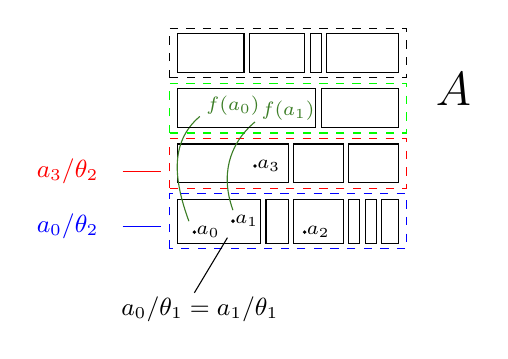
\begin{tikzpicture}[scale=.7]
\uncover<5->{      \draw[dashed,blue] (-.15,0.1) rectangle (4.15,1.1);
      \draw[dashed,red] (-.15,1.2) rectangle (4.15,2.1);
      \draw[dashed,green] (-.15,2.2) rectangle (4.15,3.1);
      \draw[dashed] (-.15,3.2) rectangle (4.15,4.1);
    }
      \draw (0,0.2) rectangle (1.5,1)
      (1.6,0.2) rectangle (2,1)
      (2.1,0.2) rectangle (3,1)
      (3.1,0.2) rectangle (3.3,1)
      (3.4,0.2) rectangle (3.6,1)
      (3.7,0.2) rectangle (4,1);
      \fill (.3,.4) circle (1pt);
      \draw[font=\scriptsize] (.55,.4) node {$a_0$};
      \fill (1,.6) circle (1pt);
      \draw[font=\scriptsize] (1.25,.6) node {$a_1$};
      \fill (2.3,.4) circle (1pt);
      \draw[font=\scriptsize] (2.55,.4) node {$a_2$};

      \draw[font=\LARGE] (5,3) node {$A$};

      \draw (0,1.3) rectangle (2,2)
      (2.1,1.3) rectangle (3,2)
      (3.1,1.3) rectangle (4,2);
      \fill (1.4,1.6) circle (1pt);
      \draw[font=\scriptsize] (1.65,1.6) node {$a_3$};

\uncover<4>{
\draw[olivegreen] (.2,.6) to [out=110, in=220] (.4,2.5);
\draw[olivegreen] (1,.8) to [out=110, in=220] (1.4,2.4);}
%\fill (.5,2.7) circle (1pt);      
\uncover<4->{
\draw[font=\scriptsize, olivegreen] (1,2.7) node {$f(a_0)$};
%\fill (1.5,2.6) circle (1pt);       
\draw[font=\scriptsize, olivegreen] (2,2.6) node {$f(a_1)$};}

\uncover<5->{ \draw[red,font=\small] (-2,1.5) node {$a_3/\theta_2$};
      \draw[red] (-1,1.5) -- (-.3,1.5);
      \draw[blue,font=\small] (-2,.5) node {$a_0/\theta_2$};
      \draw[blue] (-1,.5) -- (-.3,.5);
}
\uncover<3->{        \draw[font=\small] (.4,-1) node {$a_0/\theta_1 = a_1/\theta_1$};
      \draw (.3,-.7) -- (.9,.3);}

      \draw (0,2.3) rectangle (2.5,3)
      (2.6,2.3) rectangle (4,3);

      \draw (0,3.3) rectangle (1.2,4)
      (1.3,3.3) rectangle (2.3,4)
      (2.4,3.3) rectangle (2.6,4)
      (2.7,3.3) rectangle (4,4);
      % \fill (3.3,3.4) circle (1pt);
      % \draw (3.55,3.4) node {$a_4$};
    \end{tikzpicture}
  \end{center}
}
\vspace{.3em}

  \[\uncover<5->{\theta_2 = (a_0, a_1, a_2, \dots | a_3, \dots | \dots ),} \quad
\uncover<2->{  \theta_1 = (a_0, a_1, \dots | a_2, a_8, \dots |a_3 \dots)}\]
}

% \uncover<6->{The set of all congruences of an algebra forms the \alert{congruence lattice} of
%   the algebra, denoted $\bCon \bA$. Insight into the structure of $\bA$ is
%   gained by knowing the shape of $\bCon \bA$. 
% }
%% 7. %%%%%%%%%%%%%%%%%%%%%%%%%%%%%%%%%%%%%%%%%%%%%%%%%%%%%%%%%%%%%%%%%%%%%%%%%%%%%
\frame[label=decompositions]{
  \frametitle{Congruence Decompositions}
  \framesubtitle{We know an algebra by the congruences it keeps.}
%%%%%%%%%%%%%%%%%%%%%%%%%%%%%%%%%%%%%%%%%%%%%%%%%%%%%%%%%%%%%%%%%%%%%%%%%%%%%%
\begin{center}
  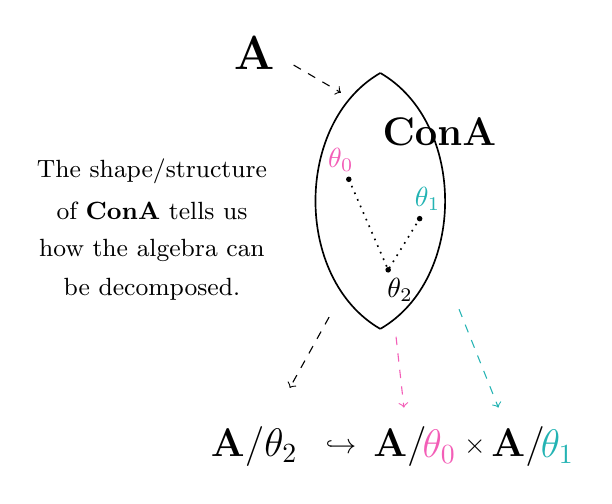
\begin{tikzpicture}[scale=.5]
    \draw[font=\LARGE] (-3.2,7) node {$\bA$};
      \uncover<2->{         
        \draw[->,dashed] (-2.2,6.7) -- (-1,6);
        \draw[->,dashed] (-1.3,.3) -- (-2.3,-1.5);
        \draw[->,dashed,CarnationPink] (.4,-.2) -- (.6,-2);
        \draw[->,dashed,TealBlue] (2,.5) -- (3,-2);}
      
      \draw[font=\Large] (1.5,5) node {$\bCon \bA$};

      \draw[font=\small] (-5.8,4) node {The shape/structure};
      \draw[font=\small] (-5.8,3) node {of $\bCon \bA$ tells us};
      \draw[font=\small] (-5.8,2) node {how the algebra can};
      \draw[font=\small] (-5.8,1) node {be decomposed.};
      
      \draw[semithick] (0,6.5) to [out=210,in=150] (0,0);% \fill (0,0) circle (2pt);
      \draw[semithick] (0,0) to [out=30,in=-30] (0,6.5);% \fill (0,6.5) circle (2pt);
      \draw[CarnationPink] (-1,4.3) node {$\theta_0$};
      \draw[TealBlue] (1.2,3.3) node {$\theta_1$};
      \draw (.5,1) node {$\theta_2$};
      \draw[semithick, dotted] (-.8,3.8) to (.2,1.5) to (1,2.8);
      \fill (-.8,3.8) circle (2pt); 
      \fill (.2,1.5) circle (2pt); 
      \fill (1,2.8) circle (2pt); 

      \uncover<2->{         
        \draw[font=\Large] (-3.2,-3) node {$\bA/\theta_2$}; 
        \draw (-1,-3) node {$\hookrightarrow$};
        \draw[font=\Large] (.5,-3) node {$\bA/$};
        \draw[font=\Large,CarnationPink] (1.5,-3) node {$\theta_0$};
        \draw (2.4,-3) node {$\times$};
        \draw[font=\Large] (3.5,-3) node {$\bA/$};
        \draw[font=\Large,TealBlue] (4.5,-3) node {$\theta_1$};
      }
    \end{tikzpicture}
  \end{center}

}

\frame[label=problem]{
  \frametitle{The Problem}
  \framesubtitle{What are the possible shapes of congruence lattices?}
  \uncover<2->{%
    \begin{theorem}[{\small Gr\"{a}tzer-Schmidt, 1963}]
      Every algebraic lattice is isomorphic to
      the congruence lattice of\\ an algebra.
    \end{theorem}
  }
  \uncover<3->{%
    Thus, there is essentially no restriction on the shape
    of a congruence lattice of an \emph{infinite} algebra.
  }
  \uncover<4->{%
    \begin{block}{What if the algebra is finite?}{}
    }
    \uncover<4->{%
      \underline{Problem}: Given a finite lattice \bL, does there exist a
      \emph{finite}
      \phantom{\underline{Problem}: }algebra \bA\ such that $\bCon\bA \cong \bL$?
    }
    \uncover<5->{%
      \begin{columns}
        \column{0mm}
        \column{108mm}
        \begin{itemize}
        \item[\underline{status}:] open
        \item[\underline{age}:] 50+ years
%        \item[\underline{difficulty}:] probably hard
        \end{itemize}
      \end{columns}
    \end{block}
  }
}% end frame: background

\frame[label=knownresults]{
  \frametitle{Known Results: {\small lattices of size $\leq 6$ are congruence lattices.}}
  % \framesubtitle{What are the possible shapes of congruence lattices?}
  
  \begin{center}
    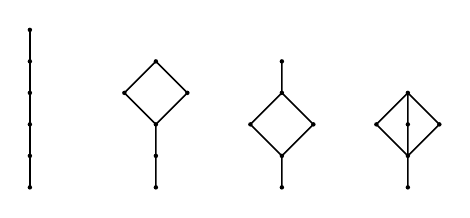
\begin{tikzpicture}[scale=.4]

      % lat1
      \foreach \j in {1,...,6}
      { \path (0,\j) coordinate (0\j); \fill (0\j) circle (2pt); }
      \draw[semithick] (01) to (06);

      % lat2
      \foreach \j in {1,2,3,5}
      { \path (4,\j) coordinate (4\j); \fill (4\j) circle (2pt); }
      \path (3,4) coordinate (34); \fill (34) circle (2pt);
      \path (5,4) coordinate (54); \fill (54) circle (2pt);
      \draw[semithick] (41) to (43) to (34) to (45) to (54) to (43);

      % lat3
      \foreach \j in {1,2,4,5}
      { \path (8,\j) coordinate (8\j); \fill (8\j) circle (2pt); }
      \path (7,3) coordinate (73); \fill (73) circle (2pt);
      \path (9,3) coordinate (93); \fill (93) circle (2pt);
      \draw[semithick] (81) to (82) to (73) to (84) to (85) (84) to (93) to (82);

      % lat4
      \foreach \j in {1,...,4}
      { \path (12,\j) coordinate (12\j); \fill (12\j) circle (2pt); }
      \path (11,3) coordinate (113); \fill (113) circle (2pt);
      \path (13,3) coordinate (133); \fill (133) circle (2pt);
      \draw[semithick] (121) to (124) to (113) to (122) to (133) to (124);
    \end{tikzpicture}
  \end{center}

  \begin{center}
    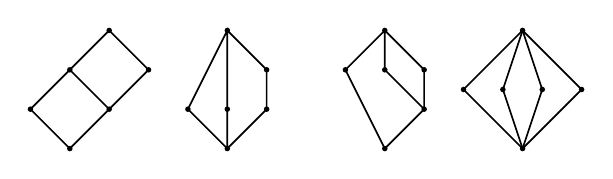
\begin{tikzpicture}[scale=.5]

      % lat5
      \path (0,1) coordinate (01); \fill (01) circle (2pt);
      \foreach \j in {0,2} 
      { \path (1,\j) coordinate (1\j); \fill (1\j) circle (2pt); }
      \foreach \j in {1,3} 
      { \path (2,\j) coordinate (2\j); \fill (2\j) circle (2pt); }
      \path (3,2) coordinate (32); \fill (32) circle (2pt);
      \draw[semithick] (10) to (01) to (23) to (32) to (10) (21) to (12);

      % lat6
      \foreach \j in {0,1,3} 
      { \path (5,\j) coordinate (5\j); \fill (5\j) circle (2pt); }
      \path (4,1) coordinate (41); \fill (41) circle (2pt);
      \foreach \j in {1,2} 
      { \path (6,\j) coordinate (6\j); \fill (6\j) circle (2pt); }
      \draw[semithick] (50) to (41) to (53) to (50) to (61) to (62) to (53);
      
      % lat7
      % \foreach \i in {7,8,9} 
      \foreach \i in {8,9,10} 
      { \path (\i,2) coordinate (\i2); \fill (\i2) circle (2pt); }
      \path (9,0) coordinate (90); \fill (90) circle (2pt);
      \path (9,3) coordinate (93); \fill (93) circle (2pt);
      \path (10,1) coordinate (101); \fill (101) circle (2pt);
      \draw[semithick] (90) to (82) to (93) to (92) to (101) to (90) (101) to (102) to (93);

      % lat8
      \foreach \j in {0,3}
      { 
        \path (12.5,\j) coordinate (125\j); 
        \fill (125\j) circle (2pt);
      }
      \foreach \i in {11,...,14}
      { 
        \path (\i,1.5) coordinate (\i15); 
        \fill (\i15) circle (2pt);
        \draw[semithick] (\i15) to (1250);
        \draw[semithick] (\i15) to (1253);
      }

    \end{tikzpicture}
  \end{center}

  \begin{center}
    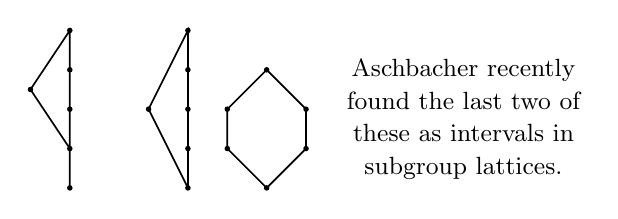
\begin{tikzpicture}[scale=.5]

      % lat9
      \foreach \j in {1,...,5}
      { \path (1,\j) coordinate (1\j); \fill (1\j) circle (2pt); }
      \path (0,3.5) coordinate (035); \fill (035) circle (2pt);
      \draw[semithick] (11) to (15) to (035) to (12);

      % lat10
      \foreach \j in {1,...,5}
      { \path (4,\j) coordinate (4\j); \fill (4\j) circle (2pt); }
      \path (3,3) coordinate (33); \fill (33) circle (2pt);
      \draw[semithick] (41) to (45) to (33) to (41);

      % lat11
      \foreach \j in {2,3}
      { \path (5,\j) coordinate (5\j); \fill (5\j) circle (2pt);
        \path (7,\j) coordinate (7\j); \fill (7\j) circle (2pt); }
      \foreach \j in {1,4} 
      { \path (6,\j) coordinate (6\j); \fill (6\j) circle (2pt);}
      \draw[semithick] (61) to (52) to (53) to (64) to (73) to (72) to (61);

      \draw[font=\small] (11,4) node {Aschbacher recently};
      \draw[font=\small] (11,3.2) node {found the last two of};
      \draw[font=\small] (11,2.4) node {these as intervals in};
      \draw[font=\small] (11,1.5) node {subgroup lattices.};
      
    \end{tikzpicture}
  \end{center}
\uncover<2->{
  {\bf Theorem:} {\it Every lattice with at most 6 elements is
    a \mbox{congruence} lattice of a finite algebra.}}
}

\frame[label=results]{
  \frametitle{Recent Results}
  \begin{center}
    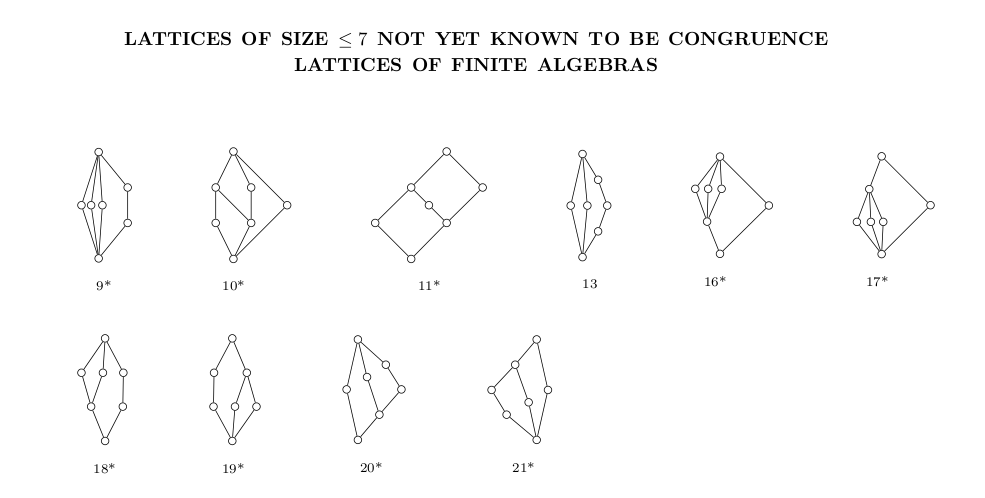
\includegraphics[height=2.5in]{Sevens}
  \end{center}
  \hfill {\small Figure courtesy of Peter Jipsen.}
}  

\frame{
  \frametitle{Recent Results}
  \begin{center}
    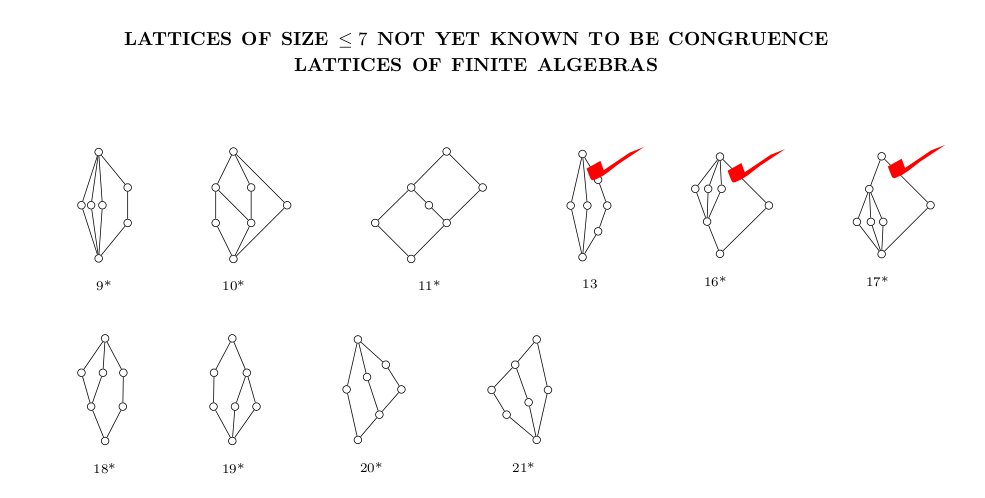
\includegraphics[height=2.5in]{Sevens1}
  \end{center}
}  

\frame{
  \frametitle{Recent Results}
  \begin{center}
    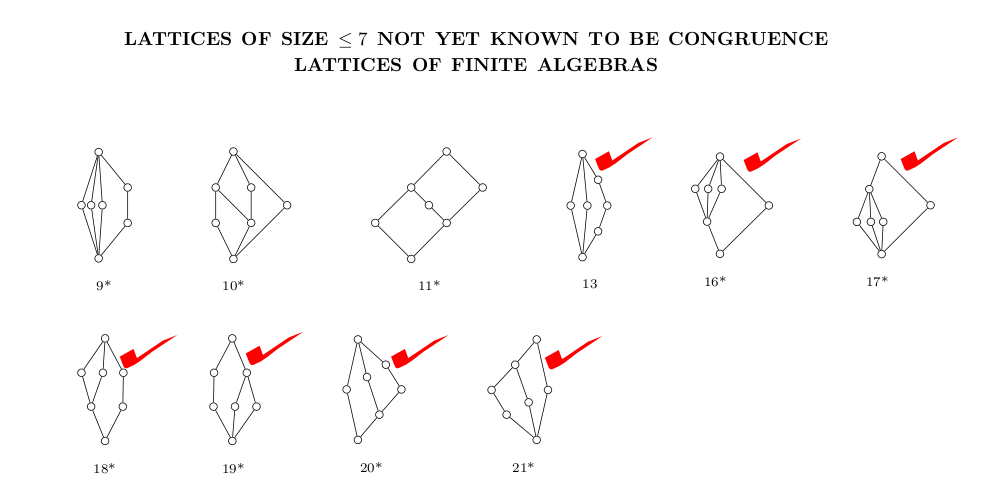
\includegraphics[height=2.5in]{Sevens2}
  \end{center}
}  

\frame{
  \frametitle{Recent Results}
  \begin{center}
    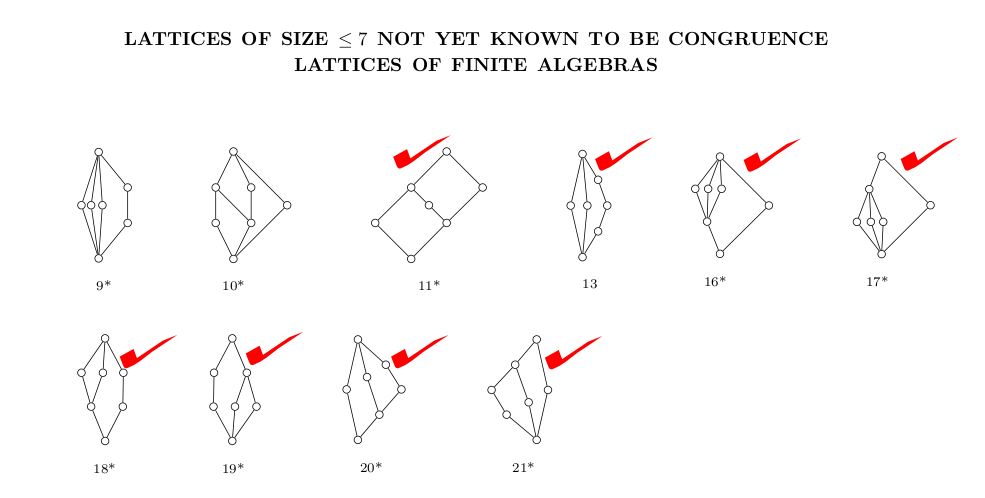
\includegraphics[height=2.5in]{Sevens3}
  \end{center}
}  

\frame{
  \frametitle{Recent Results}
  \begin{center}
    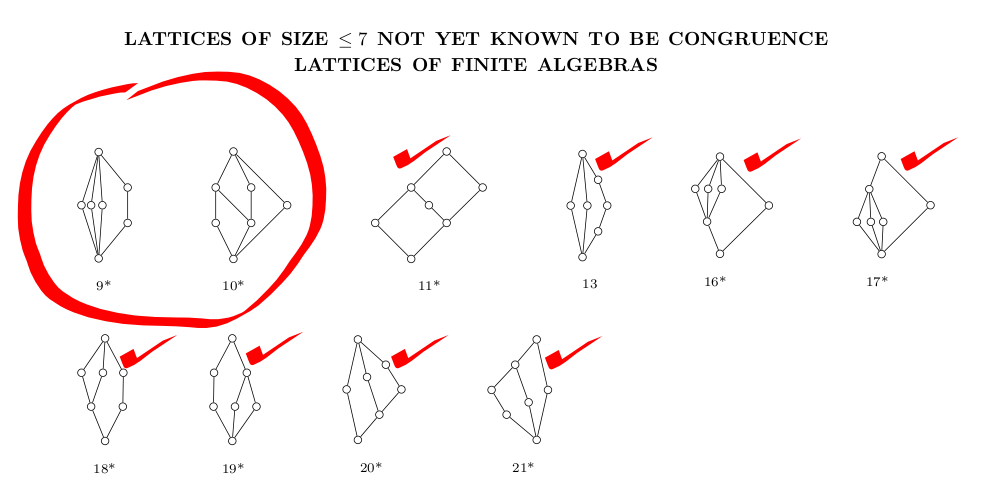
\includegraphics[height=2.5in]{Sevens4}
  \end{center}
}  

\frame{
\frametitle{}
\begin{center}

\includegraphics[height=2in]{thankyougreen2}
%\includegraphics[height=2in]{mahalopebbles}
\end{center}
}
\frame{
\frametitle{}
\begin{center}
%
\includegraphics[height=2in]{thankyougreen2}

\includegraphics[height=2in]{mahalo}
\end{center}
}




\end{document}


%%%%%%%%%%%%%%%%%%%%%%%% END DOCUMENT %%%%%%%%%%%%%%%%%%%%%%%%%%%%%%%%%%%
%%%%%%%%%%%%%%%%%%%%%%%% END DOCUMENT %%%%%%%%%%%%%%%%%%%%%%%%%%%%%%%%%%%
%%%%%%%%%%%%%%%%%%%%%%%% END DOCUMENT %%%%%%%%%%%%%%%%%%%%%%%%%%%%%%%%%%%
%%%%%%%%%%%%%%%%%%%%%%%% END DOCUMENT %%%%%%%%%%%%%%%%%%%%%%%%%%%%%%%%%%%
